\documentclass{article}
\usepackage[utf8]{inputenc}
\usepackage[spanish,mexico]{babel}
\usepackage{mathtools}
\usepackage{amsmath}
\usepackage{enumerate}
\usepackage{float}


\begin{document}
\author{Luciano Andrade}
\title{Simulación de Sistemas Continuos - Práctica 2}
\maketitle

\begin{itemize}

%%%%%%%%%%%%%%%%%%%%%%%%%%%%%%%%%%%%%%%%%%%%%%%%%%%%%%%%%%%%%%%%%%%%%%%%%%%%%%%
  \item[P2.1] Estabilidad Marginal : Dado el siguiente sistema lineal y estacionario

\begin{align}
\dot{x} &= \begin{pmatrix}
  1250 & -25113 & -60050 & -42647 & -23999 \\
   500 & -10068 & -24057 & -17092 &  -9613 \\
   250 &  -5060 & -12079 &  -8586 &  -4826 \\
  -750 &  15101 &  36086 &  25637 &  14420 \\
   250 &  -4963 & -11896 &  -8438 &  -4756 
       \end{pmatrix} 
\cdot x +
\begin{pmatrix}
	5 \\
	2 \\
	1 \\
	-3 \\
 	1
	\end{pmatrix}
\cdot u 
%\notag \\
%y &= \begin{pmatrix}-1 & 26 & 59 & 43 & 23 \end{pmatrix} \cdot x
 \label{P2.1a} \tag{P2.1a}
\end{align}

con condiciones iniciales:

\begin{equation}
x_0 = \begin{pmatrix}1 & -2 & 3 & -4 & 5 \end{pmatrix}^{T}
 \label{P2.1b} \tag{P2.1b}
\end{equation}

Determinar el paso de integración, $h_{marg}$, para el cual FE dará resultados marginales estables.
Simular el sistema durante 10 segundos de tiempo de simulación con una entrada escalón utilizando el método de FE con los siguientes pasos  de integración : (i) $h=0.1 \cdot h_{marg}$, (ii) $h=0.95 \cdot h_{marg}$, (iii) $h= h_{marg}$, (iv) $h= 1.05 \cdot h_{marg}$ y (v) $h=2 \cdot h_{marg}$. Discutir los resultados

rta :
El vector de autovalores es 
\begin{equation*}
\begin{pmatrix}
  - 4 + 3.i  \\
  - 4 - 3.i  \\
  - 5        \\
  - 2        \\
  - 1   
	\end{pmatrix}
\end{equation*}
entonces $h_{marg} < 0.32$

\begin{figure}[H]
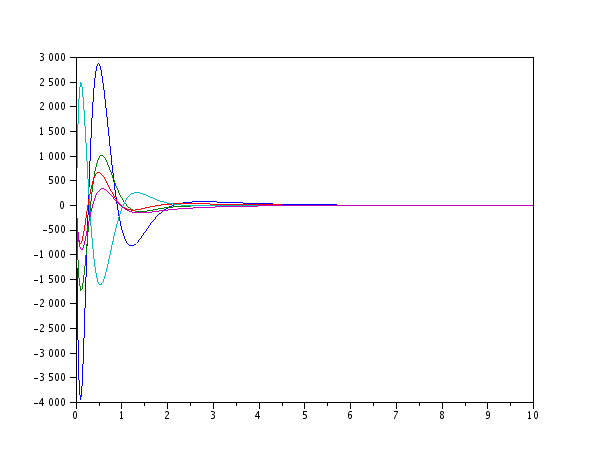
\includegraphics[width=\textwidth]{img/ej2-1-i.png}
\caption{$h=0.1 \cdot h_{marg}$}
\end{figure}

\begin{figure}[H]
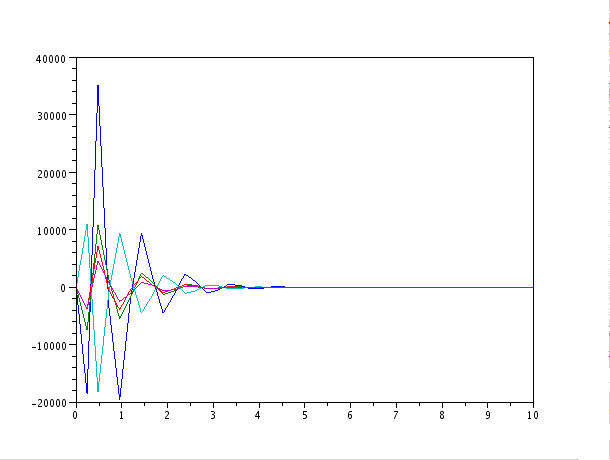
\includegraphics[width=\textwidth]{img/ej2-1-ii.png}
\caption{$h=0.95 \cdot h_{marg}$}
\end{figure}

\begin{figure}[H]
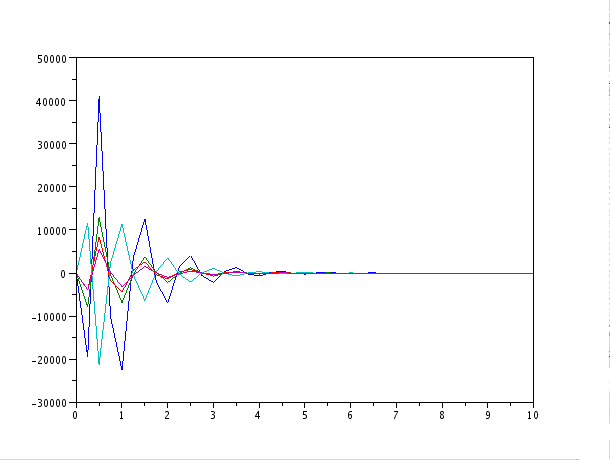
\includegraphics[width=\textwidth]{img/ej2-1-iii.png}
\caption{$h=h_{marg}$}
\end{figure}

\begin{figure}[H]
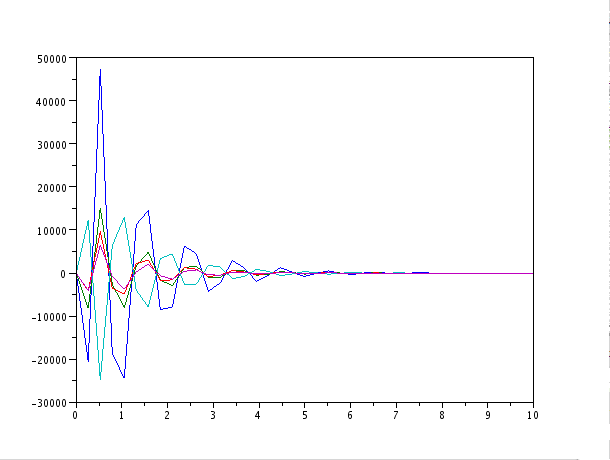
\includegraphics[width=\textwidth]{img/ej2-1-iv.png}
\caption{$h=1.05 \cdot h_{marg}$}
\end{figure}

\begin{figure}[H]
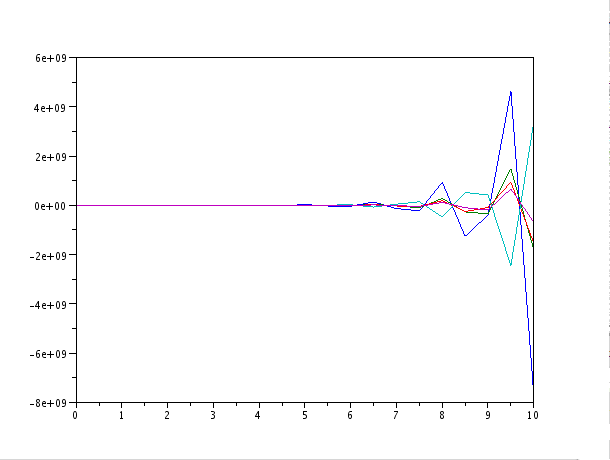
\includegraphics[width=\textwidth]{img/ej2-1-v.png}
\caption{$h=2 \cdot h_{marg}$}
\end{figure}

%%%%%%%%%%%%%%%%%%%%%%%%%%%%%%%%%%%%%%%%%%%%%%%%%%%%%%%%%%%%%%%%%%%%%%%%%%%%%%%

  \item[P2.2] Precisión de Integración : Para el sistema del Prob.[P2.1], determinar el máximo paso de integración que permite obtener una precisión global del $1\%$
Para esto , primero hay que obtener la solución analitica del sistema y luego simularlo utilizando el método de FE (durante 10 segundos), hasta obtener que ambas soluciones difieran $1\%$:
\begin{equation}
\varepsilon_{global} = \frac{\|x_{anal} - x_{num}\|}{\|x_{anal}} \leq 0.01
 \label{P2.2a} \tag{P2.2a}
\end{equation}

Repetir el mismo experimento con el método BE. Dado que el mismo sistema es lineal, se permite calcular la matrix F utilizando la inversión matricial.

Para FE $ h = 0.001 $ $\varepsilon_{global} \approx 0.0071622$.
Para BE $ h = 0.001 $ $\varepsilon_{global} \approx 0.0070922$ 
%%%%%%%%%%%%%%%%%%%%%%%%%%%%%%%%%%%%%%%%%%%%%%%%%%%%%%%%%%%%%%%%%%%%%%%%%%%%%%%
\item [P2.3] Método Blending: Dado el siguiente sistema lineal y estacionario: 

\begin{equation}
	\dot{x} = 
		\begin{pmatrix}
			0 & 1 \\
			-9.01 & 0.2 
		\end{pmatrix}
	\cdot x %+ 
		%\begin{pmatrix}
		%	0 \\ 1
		%\end{pmatrix}
	%\cdot u 
 \label{P2.3a} \tag{P2.3a}
	%y &= \begin{pmatrix} 0 & 1 \end{pmatrix} \cdot x + 2 \cdot u 
\end{equation}

con condicion inicial

\begin{equation}
x_0 = \begin{pmatrix} 1 & -2\end{pmatrix}^T
 \label{P2.3b} \tag{P2.3b}
\end{equation}

Encontrar la solución analítica. Simulando durante 25 segundos, determinar el máximo paso de integración que permite alcanzar una precisión global del $1\%$ utilizando FE. Luego repetir para BE. Sacar conclusiones
Un algoritmo mixto puede obtenerse de la siguiente forma: hacemos un paso de integración FE y luego el mismo paso lo hacemos con BE, y damos como resultado el promedio de ambos valores. Para este método mixto, obtener el máximo paso que permite alcansar una precisión del $1\%$. Comparar el resultado con el de FE y BE por sí mismo.

Para FE $h = 0.001$ $\varepsilon \approx 0.0071622$, para BE y $h = 0.001$ $\varepsilon \approx 0.0092752 $ 
Con $h = 0.01$ para el algoritmo mixto $\varepsilon \approx 0.0188726$.
%%%%%%%%%%%%%%%%%%%%%%%%%%%%%%%%%%%%%%%%%%%%%%%%%%%%%%%%%%%%%%%%%%%%%%%%%%%%%%%
\item[P2.4] Método Ciclico. Repetir el Prob.[P2.3]. Sin embargo, esta vez utilizaremos otro algorimo. En lugar de utilizar el promedio de FE y BE, alternaremos un paso con FE y otro con BE. Tales algorimos se llaman métodos cíclicos.
Determinar nuevamente el máximo paso de integración que alcanzze un $1\%$ de precisión y comparar con lo métodos de FE y BE.

Para el algorimos cíclico $h = 0.01$ $\varepsilon \approx 0.0188583$.

%%%%%%%%%%%%%%%%%%%%%%%%%%%%%%%%%%%%%%%%%%%%%%%%%%%%%%%%%%%%%%%%%%%%%%%%%%%%%%%
\item[P2.5] Dominio de estabilidad : Métodos mixtos y cíclicos. Obtener el dominio de estabilidad para el método míxto del Prob.[2.3]. ¿Que puede concluirse al comparar dichos dominios de estabilidad con los de FE y BE? ¿Cómo se puede explicar a partir de estos dominios de estabilidad los resultados de Prob.[P2.3]?
Repetir el análisis para el método cíclico del Prob.[P2.4]. Para analizar el dominio de estabilidad en este último caso, puede utilizar la siguiente ayuda:
En lugar de interpretar este método cíclico como la conmutación de dos métodos tras cada paso, puede pensar que consite en un simple paso grande formado por dos pequeños:
\begin{align}
	x(k+0.5) &= x(k) \cdot 0.5 + h \cdot \dot{x}(k) \tag{P2.5a} \\
	x(k+1)   &= x(k + 0.5) + 0.5 \cdot h \cdot \dot{x}(k+1) \tag{P2.5b}
\end{align}

\begin{figure}[H]
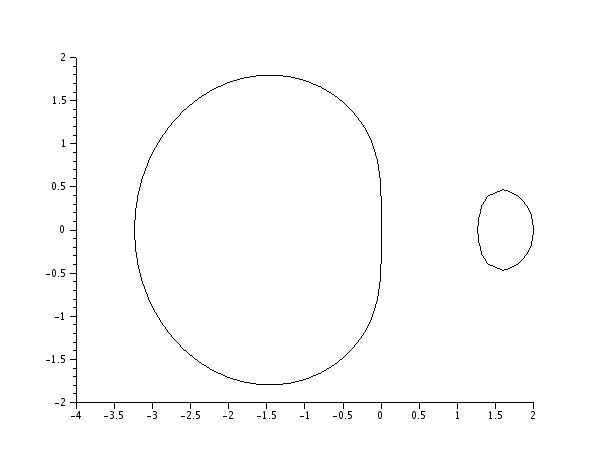
\includegraphics[width=\textwidth]{img/ej5-mixto.png}
\caption{Mixto}
\end{figure}

\begin{figure}[H]
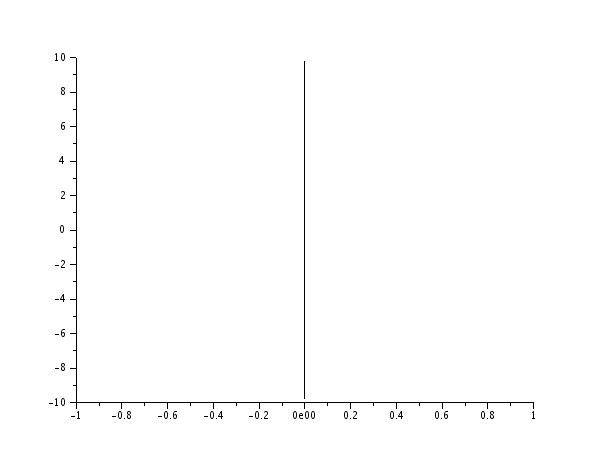
\includegraphics[width=\textwidth]{img/ej5-ciclico.png}
\caption{Cíclico}
\end{figure}

%%%%%%%%%%%%%%%%%%%%%%%%%%%%%%%%%%%%%%%%%%%%%%%%%%%%%%%%%%%%%%%%%%%%%%%%%%%%%%%
\item[P2.6] Ajuste del Dominio de Estabilidad: Método Mixto : Veremos otro método derivado del método mixto antes analizado. Aqui, en lugar de utilizar el promedio de FE y BE, utilizaremos el promedio ponderado:
\begin{equation}
x(k+1) = \vartheta \cdot \boldsymbol{X_{FE}}(k + 1) + (1 - \vartheta) \cdot \boldsymbol{X_{BE}}(k + 1)
\tag{P2.6a}
\end{equation}
Este método se denomina método-$\vartheta$ . Dibujar los dominios de estabilidad del método para

\begin{equation}
\vartheta = \{0, 0.1, 0.2, 0.24, 0.249, 0.25, 0.251, 0.26, 0.3, 0.5, 0.8, 1\} \tag{P2.6b}
\end{equation}

\begin{figure}[H]
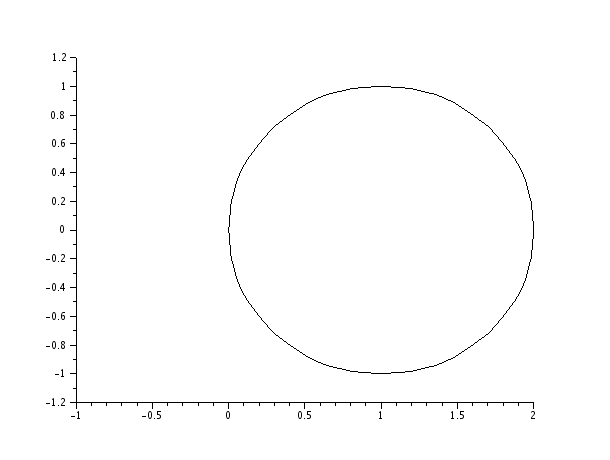
\includegraphics[width=\textwidth]{img/ej6-1.png}
\caption{$\vartheta = 0$ Backward Euler}
\end{figure}

\begin{figure}[H]
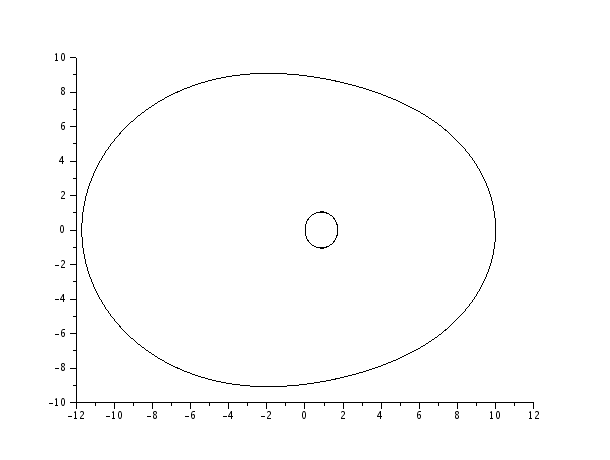
\includegraphics[width=\textwidth]{img/ej6-2.png}
\caption{$\vartheta = 0.1$ }
\end{figure}

\begin{figure}[H]
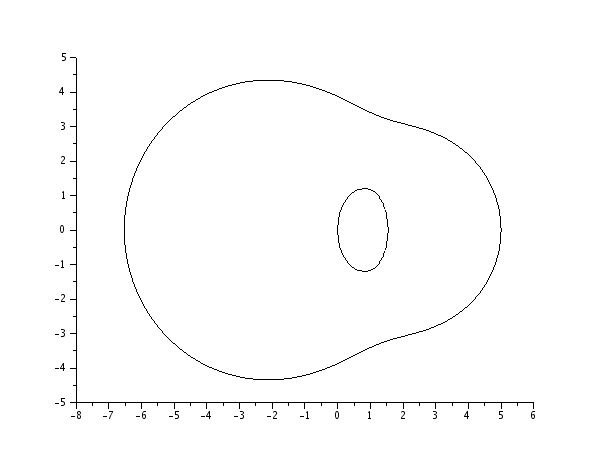
\includegraphics[width=\textwidth]{img/ej6-3.png}
\caption{$\vartheta = 0.2$ }
\end{figure}

\begin{figure}[H]
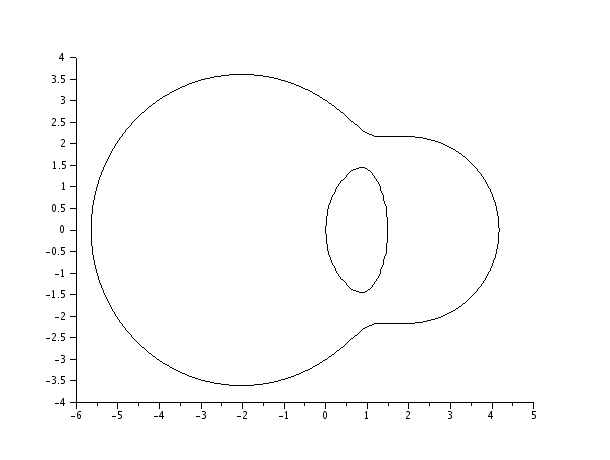
\includegraphics[width=\textwidth]{img/ej6-4.png}
\caption{$\vartheta = 0.24$ }
\end{figure}

\begin{figure}[H]
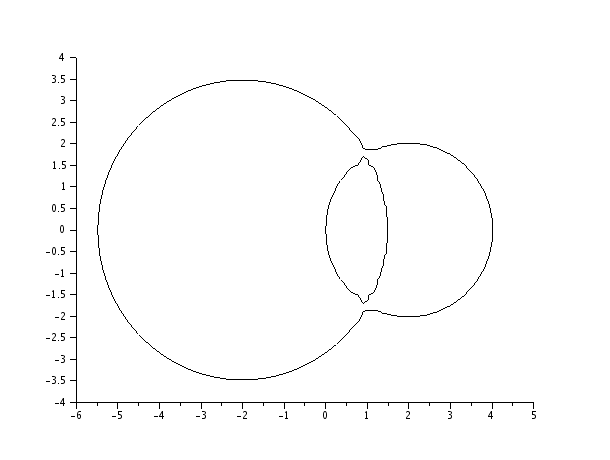
\includegraphics[width=\textwidth]{img/ej6-5.png}
\caption{$\vartheta = 0.249$ }
\end{figure}

\begin{figure}[H]
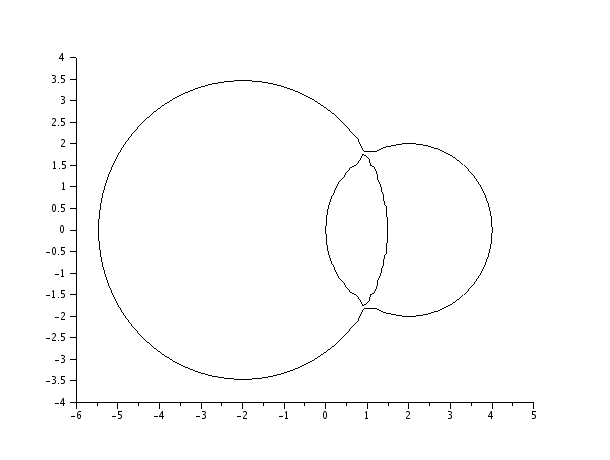
\includegraphics[width=\textwidth]{img/ej6-6.png}
\caption{$\vartheta = 0.25$ }
\end{figure}

\begin{figure}[H]
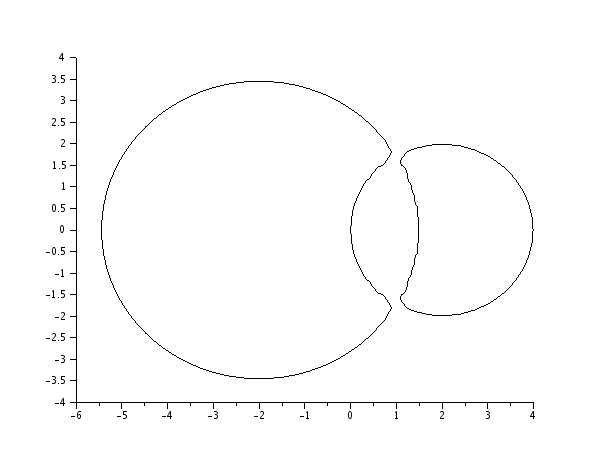
\includegraphics[width=\textwidth]{img/ej6-7.png}
\caption{$\vartheta = 0.251$ }
\end{figure}

\begin{figure}[H]
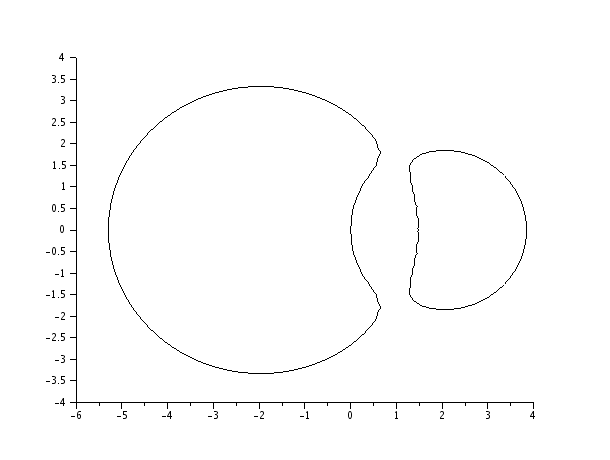
\includegraphics[width=\textwidth]{img/ej6-8.png}
\caption{$\vartheta = 0.26$ }
\end{figure}

\begin{figure}[H]
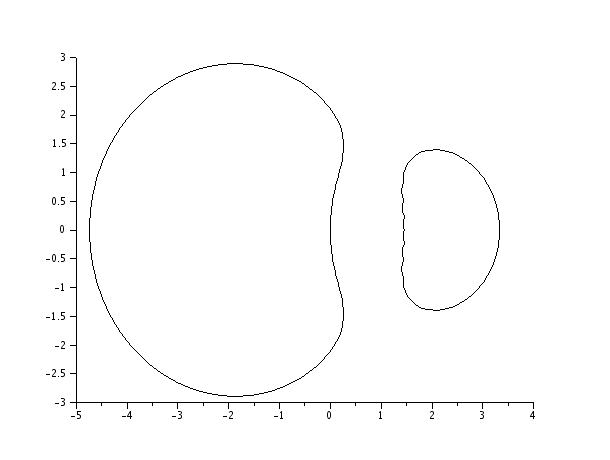
\includegraphics[width=\textwidth]{img/ej6-9.png}
\caption{$\vartheta = 0.3$ }
\end{figure}

\begin{figure}[H]
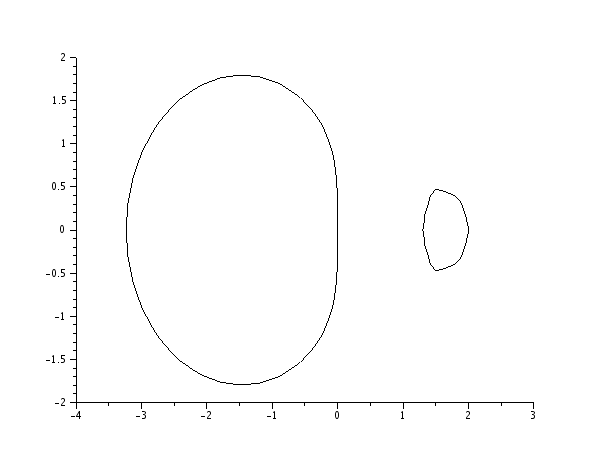
\includegraphics[width=\textwidth]{img/ej6-10.png}
\caption{$\vartheta = 0.5$ Método Mixto}
\end{figure}

\begin{figure}[H]
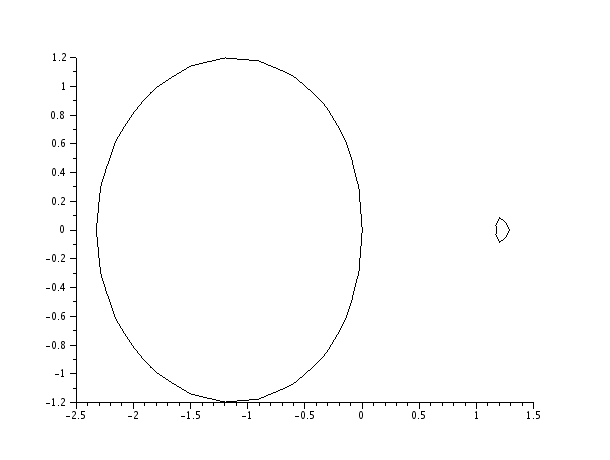
\includegraphics[width=\textwidth]{img/ej6-11.png}
\caption{$\vartheta = 0.8$}
\end{figure}

\begin{figure}[H]
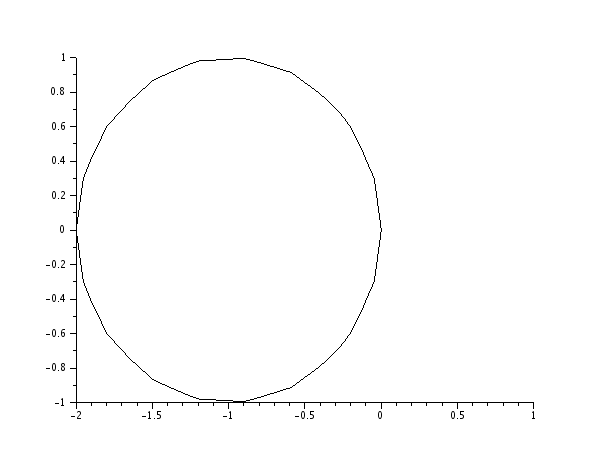
\includegraphics[width=\textwidth]{img/ej6-12.png}
\caption{$\vartheta = 1$ Forward Euler}
\end{figure}

%%%%%%%%%%%%%%%%%%%%%%%%%%%%%%%%%%%%%%%%%%%%%%%%%%%%%%%%%%%%%%%%%%%%%%%%%%%%%%%
\item[P2.7] Ajuste del Dominio de Estabilidad: Método Cíclico Veremos ahora otro método-$\vartheta$. Esta vez, a partir de un método cíclico. El parámetro que variaremos es la longitud de los dos semi-pasos de la siguiente forma:


\begin{align}
	x(k+\vartheta) &= x(k) \cdot \vartheta + h \cdot \dot{x}(k) \tag{P2.7a} \\
	x(k+1)   &= x(k + \vartheta) + \vartheta \cdot h \cdot \dot{x}(k+1) \tag{P2.7b}
\end{align}


Se pide entonces determinar el parámetro $\vartheta$ tal que el método tenga una región de estabilidad similar a BE, pero donde el borde de la estabilidad sobre el eje real positivo del pano $(\lambda \cdot h)$ esté localizado en $+10$ en lugar de $+2$.
Dibujar el dominio de estabilidad para este método

\begin{figure}[H]
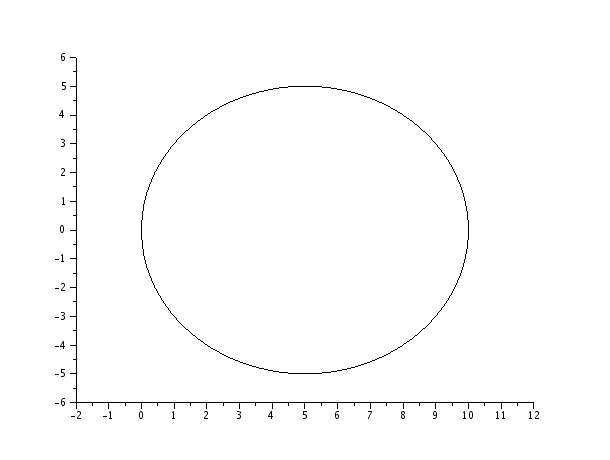
\includegraphics[width=\textwidth]{img/ej7.png}
\caption{$\vartheta = 0.4$}
\end{figure}



%%%%%%%%%%%%%%%%%%%%%%%%%%%%%%%%%%%%%%%%%%%%%%%%%%%%%%%%%%%%%%%%%%%%%%%%%%%%%%%
\end{itemize}
\end{document}
